% I only need the arrows for this one.
%\usepackage{tikz}
%\usetikzlibrary{arrows}
% Place the TikZ picture in a figure environment.
%\begin{figure}
%\centerline{

% Resize it to 5cm wide.
  \resizebox{.3\linewidth}{!}{
  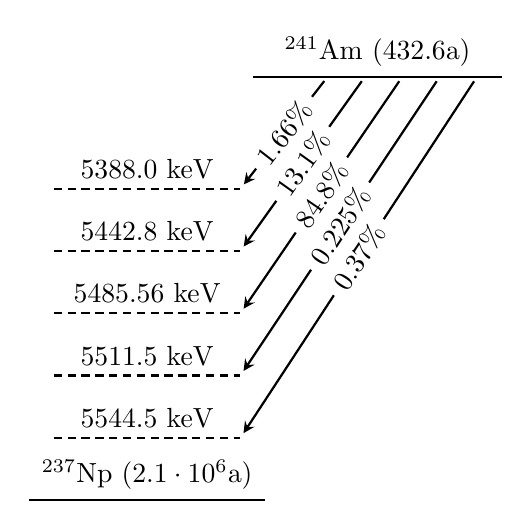
\begin{tikzpicture}[
      scale=0.45,
      level/.style={thick},
      virtual/.style={thick,densely dashed},
      trans/.style={thick,->,shorten >=2pt,shorten <=2pt,>=stealth},
      classical/.style={thin,double,<->,shorten >=4pt,shorten <=4pt,>=stealth}
    ]
    % Draw the energy levels.
    \draw[level] (20em,18em)    -- (40em,18em) node[midway,above] {$^{241}$Am (432.6a)};
    \draw[level] (2em,-16em)  -- (21em,-16em) node[midway,above] {$^{237}$Np ($2.1\cdot10^6$a)};
    % Draw the virtual levels.
    \draw[virtual] (4em,9em)  -- (19em,9em)  node[midway,above] {5388.0 keV};
    \draw[virtual] (4em,4em)  -- (19em,4em)  node[midway,above] {5442.8 keV};
    \draw[virtual] (4em,-1em) -- (19em,-1em) node[midway,above] {5485.56 keV};
    \draw[virtual] (4em,-6em) -- (19em,-6em) node[midway,above] {5511.5 keV};
    \draw[virtual] (4em,-11em) -- (19em,-11em) node[midway,above] {5544.5 keV};
    % Draw the transitions.
    \draw[trans] (26em, 18em) -- node[sloped,fill=white] {$1.66\%$}  (19em, 9em);
    \draw[trans] (29em, 18em) -- node[sloped,fill=white] {$13.1\%$} (19em, 4em);
    \draw[trans] (32em,18em) -- node[sloped,fill=white] {$84.8\%$}  (19em,-1em);
    \draw[trans] (35em,18em) -- node[sloped,fill=white] {$0.225\%$}  (19em,-6em);
    \draw[trans] (38em,18em) -- node[sloped,fill=white] {$0.37\%$}  (19em,-11em);
    %    \draw[classical] (4.5em,-8em) -- (1.5em,-5em) node[midway,below] {\Ga{}};
    \end{tikzpicture}
  }
%}
%\caption{Zerfallsschema Alphazerfalll von $^{241}$Am.}
%\end{figure}

%  http://www.nndc.bnl.gov/nudat2/decaysearchdirect.jsp?nuc=241AM&unc=nds
%  Author: M. S. Basunia   Citation:Nuclear Data Sheets 107, 3323 (2006)
%  Half-Life: 432.6
%  Alphas:
%  Energy (keV)   Intensity (%)   Dose ( MeV/Bq-s )
%    4758         5E-6 % 5    2.4E-7 24 
%    4800         8.6E-5 %   4.128E-6
%    4834         7E-4 %   3.384E-5
%    5004         1E-4 %   5.004E-6
%    5068         1.4E-4 %   7.0952E-6
%    5089         4.0E-4 % 4    2.04E-5 20 
%    5096         4.0E-4 % 4    2.04E-5 20 
%    5114         4E-4 %   2.0456E-5
%    5137         3.2E-4 %   1.644E-5
%    5155         7E-4 %   3.609E-5
%    5178         3E-4 %   1.553E-5
%    5182         9E-4 %   4.664E-5
%    5192         6E-4 %   3.115E-5
%    5217         1.0E-5 % 10    5E-7 5 
%    5223         0.0013 %   6.79E-5
%    5244         0.0024 %   1.259E-4
%    5279         5E-4 %   2.64E-5
%    5322         0.015 % 5    8E-4 3 
%  * 5388         1.660 % 20    0.0894 11 
%    5416.5       0.0100 % 10    5.4E-4 5 
%  * 5442.80 13   13.1 % 3    0.713 16 
%    5469         0.020 % 20    0.0011 11 
%  * 5485.56 12   84.8 % 5    4.65 3 
%  * 5511.5       0.225 % 5    0.0124 3 
%  * 5544.5  16   0.37 % 3    0.0205 17
